\documentclass[12pt]{article}

\usepackage{times}
\usepackage{epsfig}
\usepackage{graphicx}
\usepackage{amsmath}
\usepackage{amssymb}
\usepackage{color, soul} 	%for highlighting
\usepackage{listings} 		%for writing code
\lstset{
basicstyle=\small\ttfamily,
columns=flexible,
breaklines=true
}
\usepackage[margin=1in]{geometry} %for margins
\setlength{\parskip}{12pt plus3pt minus3pt} %for paragraph spacing

\setcounter{page}{1}
\begin{document}

\begin{titlepage}

\title{Space Brain - Investigating the Suitability of an FPGA-based Convolutional Neural Network for Space Applications}
\author{Jukka (Jacobus) Hertzog}
\def\supervisor{Dr. Felix Winterstein}
\def\secondmarker{Dr. David Thomas}
\def\course{EE4T}
\def\cid{00828711}

\setlength{\parindent}{0pt}
\setlength{\parskip}{0pt}
\fontfamily{phv}\selectfont
{
\large
\raggedright
Imperial College London\\[17pt]
Department of Electrical and Electronic Engineering\\[17pt]
Final Year Project Interim Report 2017\\[17pt]
}
\rule{\columnwidth}{3pt}
\vfill
\centering
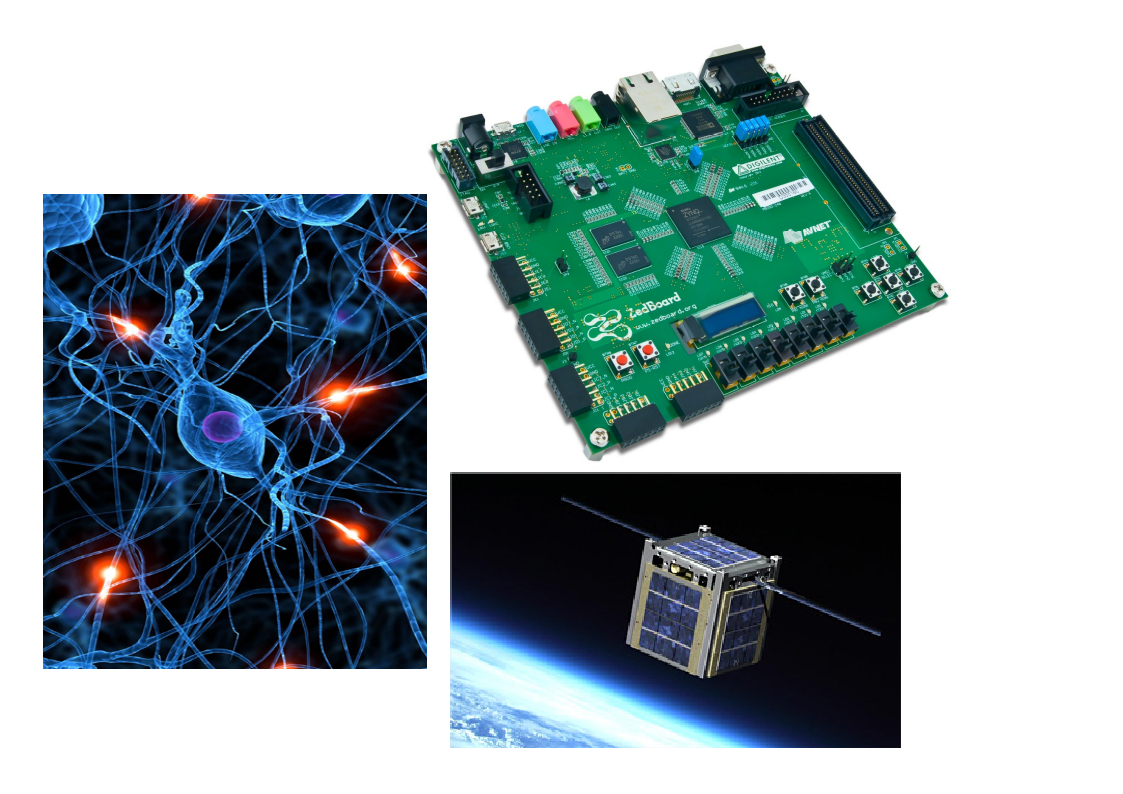
\includegraphics[width=\columnwidth,keepaspectratio]{../figures/frontCover}
\vfill
\setlength{\tabcolsep}{0pt}


\makeatletter
\begin{tabular}{p{40mm}p{\dimexpr\columnwidth-40mm}}
Project Title: & \textbf{\@title} \\[12pt]
Student: & \textbf{\@author} \\[12pt]
CID: & \textbf{\cid} \\[12pt]
Course: & \textbf{\course} \\[12pt]
Project Supervisor: & \textbf{\supervisor} \\[12pt]
Second Marker: & \textbf{\secondmarker} \\
\end{tabular}
\end{titlepage}

\section{Introduction}
\label{sec:Intro}
\vspace{-12pt}

Inspired by the structure of the optical nervous system in animals, a neural network is made up of layers of artificial neurons that recognise certain features from the input data. The idea of an artificial neural network was first introduced in 1980 \cite{neocognitron}, and driven by increases in computing power and a growth in machine learning applications, neural networks have become very powerful tools. In the last decade, the development of Convolutional Neural Networks (CNNs) has lead to great advancements in image classification accuracy.

CNNs are a powerful Deep Learning tool that can be used to solve extremely complex computational problems. In particular, they have gained popularity in image classification applications \cite{ImageNetChallenge}. Other popular applications within machine vision include video classification, face detection and gesture recognition. They are also being used in a wide range of other fields including speech recognition, natural language processing and text classification.

However, whilst achieving exceptional performance, CNNs are extremely computation and resource heavy. Typically, they will be implemented on large servers or on GPU based systems to accomodate the need for computational power. As a result, implementing them on embedded systems, which typically have very limited resources, presents many challenges. A promising solution to this problem is the use of an FPGA, which provide a very high computational efficiency with low power usage, in addition to other benefits.

Now suppose that the FPGA based CNN will be implemented on a sattelite. In orbit, the satellite will be exposed to intense raditiation, and as a result, errors will be produced on the FPGA. Before such a satellite could be designed and launched, it is important to know how these errors would affect the performance of the CNN, and if the CNN could be designed in such a way that could mitigate the impact of these errors. Therefore, the aim of this project is to implement a CNN on an FPGA-based system, and then to investigate the suitability of this system for space applications.

\vspace{-12pt}
\subsection{Report Structure}
\label{sec:Intro-Structure}
\vspace{-12pt}

The rest of the report is organised as follows. Section\ref{sec:Background} will describe the key concepts underlying the project. Section \ref{sec:ProjSpec} will lay out the project specification, and the motivation for the project. Section \ref{sec:ImpPlan} will go into detail about how the project will be implemented, including a rough time line. Finally, section \ref{sec:EvalPlan} will describe the metrics through which the project will be evaluated.

\section{Background}
\label{sec:Background}
\vspace{-12pt}

This section will provide some details and information that will provide context to the project, and will be useful for understanding key concepts in the rest of the report.

\subsection{Target Platform}
\label{sec:Background-TargetPlatform}
\vspace{-12pt}

The hardware used in this project is a product from Xilinx called a Zedboard, a development board for the Zynq-7000 System On a Chip (SoC). This board was chosen because of its useful hardware features and its integrated support for useful Xilinx proprietary tools. These tools include High Level Synthesis systems, SoC design tools and the Soft Error Mitigation IP core. The Zynq-7000 consists of a Xilinx FPGA as its Programmable Logic, and a dual-core Cortex-A9 ARM processor as its Processing System integrated together. The ARM processor facilitates easy control of the system, whilst the FPGA will be able to efficiently perform heavy computations.

\subsection{Convolutional Neural Networks}
\label{sec:Background-CNN}
\vspace{-12pt}

CNNs can be used to classify images in a forward inference process. But before using the CNN for any task, one should first train the CNN on a set of training data. The training of a CNN is usually implemented on large servers with a huge computational capacity, with an enormous set of training data. For the embedded FPGA platform, I only focus on accelerating the inference process of a CNN, and not on the training process.

A typical CNN consists of a number of layers that run in sequence. Convolution (CONV), activation function, pooling, and Fully Connected (FC) layers make up a typical CNN model, with CONV and FC being the most important. CONV and FC layers have parameters of called weights, which are set by the training process. These wieghts will determine which patterns each layer of the CNN will be activated by, and ultimately, what the CNN is able to recognise and classify. 

The first layer of a CNN reads an input image and outputs a series of feature maps. The input image will be three dimensional - the height and width of the image make up two dimensions, and colours make up the third layer. For an RGB image, the input will have a depth of 3. Then there will be CONV layers interspersed by activation function and pooling layers, which will make up most of the CNN. These layers will decompose the image into feature maps, varying from low-level features such as edges, lines, curves, etc., in the initial layers to high-leve features in the deeper layers \cite{fpgaCnnAccelerator}. Each subsequent layer reads the feature maps generated by preceding layers and generates new feature maps at its output. Finally a classifier, consisting of at least one FC layer, reads the final feature maps and determines the probability of the input imaging belonging to each category of the training data. A example of a CNN model is shown in Figure \ref{fig:typicalCNN}.
\begin{figure}

\centering
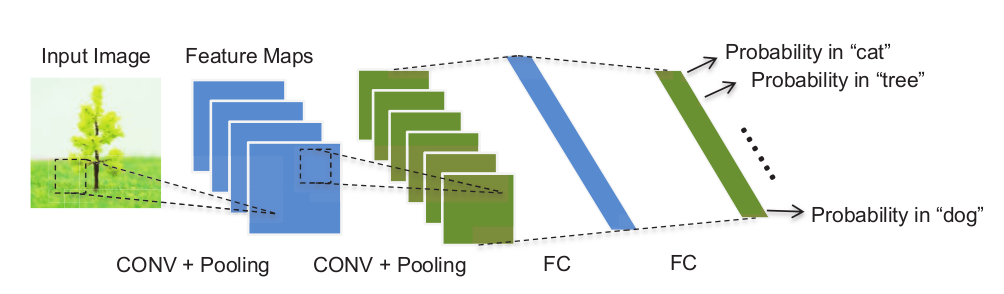
\includegraphics[width=0.75\textwidth]{../figures/typicalCnn}

  \caption{A typical CNN structure from the feature map perspective \cite{embeddedFpgaCnn} \label{fig:typicalCNN}}

\end{figure}

\subsubsection{Convolution Layer}
\label{sec:Background-CNN-Conv}
\vspace{-12pt}

The CONV layer takes a series of feature maps as input and convolves with convolutional kernels to obtain the output feature maps. It involves 3-dimensional multiply and accumulate operation of $N_{if}$ input features with $K\times K$ convolution kernels to get an output feature neuron value as shown in Equation \ref{eq:ConvLayer}
\begin{equation}
out(f_o,x,y)=\sum^{N_{if}}_{f_i=0} \sum^{K}_{k_x=0} \sum^{K}_{k_y=0} wt(f_o,f_i,k_x,k_y)\times in(f_i,x+k_x,y+k_y)
\label{eq:ConvLayer}
\end{equation}
where $out(f_o,x,y)$ and $in(f_i,x,y)$ represent the neurons at position $(x,y)$ in the feature maps $f_o$ and $f_i$, respectively and $wt(f_o,f_i,k_x,k_y)$ is the weights at position $(k_x,k_y)$ that gets convolved with input feature map $f_i$ to get the output feature map $f_o$\cite{fpgaCnnAccelerator}.

\subsubsection{Activation Functions}
\label{sec:Background-CNN-Activation}
\vspace{-12pt}

CONV layers are followed by an activation functon layer. This layer can be thought of as a decision, based on the output of the CONV layer, on to what extent each neuron in the next layer has been activated. The CONV layer output is a linear combination of the inputs and the weights at a position in the network, and role of the activation function is to produce a non-linear decision boundary. The commonly used activation functions in traditional neural networks are non-linear functions such as tanh and sigmoid, which require a longer training time in CNNs \cite{AlexNet}. Hence, Rectified Linear Unit (ReLU), defined as $y = max(x,0)$, has become the popular activation function among CNN models as it converges faster in training, and has less computational complexity than exponent functions in tanh and sigmoid, also aiding hardware design.

\subsubsection{Pooling Layer}
\label{sec:Background-CNN-Pool}
\vspace{-12pt}

Spatial pooling or subsampling is utilized to reduce the feature dimensions as we traverse deeper into the network. As shown in Equation \ref{eq:Pool}, pooling computes the maximum or average of neighboring $K\times K$ neurons in the same feature map, which also provides a form of translational invariance \cite{PoolAnalysis}. The pooling layer helps abstract higher-level features without redundancy, as well as reducing the dimensionality of lower-level features without losing important information\cite{fpgaCnnAccelerator}.
\begin{equation}
out(f_o,x,y)=\underset{0\geqslant (k_x,k_y)<K}{max/average}(in(f_o,x+k_x,y+k_y))
\label{eq:Pool}
\end{equation}

\subsubsection{Fully Connected Layer}
\label{sec:Background-CNN-FC}
\vspace{-12pt}

An FC layer is a classification layer where all the input features $(N_{if})$ are connected to all of the output features $(N_{of})$ through synaptic weights $(wt)$. These are at the end of the CNN and perform the final classification, based on the features that have been recognised by the rest of the network. Each output neuron is the weighted summation of all the input neurons as shown in Equation \ref{eq:FullyConnected}\cite{fpgaCnnAccelerator}.
\begin{equation}
out(f_o)=\sum^{N_{if}}_{f_i=0}wt(f_o,f_i)\times in(f_i)
\label{eq:FullyConnected}
\end{equation}
The outputs of the inner-product layer traverse through ReLU based activation function to the next inner-product layer or directly to a Softmax function that converts them to probability in the range (0, 1). The final accuracy layer compares the labels of the top probabilities from softmax layer with the actual label and gives the accuracy of the CNN model\cite{fpgaCnnAccelerator}.

\subsection{CNNs Implemented on FPGAs}
\label{sec:Background-CNNsImplementedOnFPGAs}
\vspace{-12pt}

CNNs are computationally demanding and consume a lot of resources, and thus are difficult to implement on an embedded systems. FPGAs are the most promising platform for the implementation of an embedded CNN, due to their high computational efficiency and low power consumption. FPGAs are also attractive because of their reconfigurability and fast development time, aided by HLS tools from FPGA vendors, which are discussed in \ref{sec:Background-HLS}. Moreover, FPGAs provide flexibility to implement the CNNs with limited data precision which reduces the memory footprint and bandwidth requirements, resulting in a better energy efficiency\cite{fpgaCnnAccelerator}.

Most research has focussed on using hardware to accelerating the computation of the CONV layers. These layers, with their  typically make up around 90\% of the CNN's computational workload. \hl{TO BE COMPLETED}

\subsection{High Level Synthesis}
\label{sec:Background-HLS}
\vspace{-12pt}

Typically, digital circuits on reconfigurable hardware architectures, such as FPGAs, are designed using a Hardware Description Language (HDL) such as Verilog of VHDL. While these methods allow the designer to have a great level of control over the system, and can produce extremely efficient designs, the designer is forced to specify functionality at a very low level of abstraction, specifying cycle by cycle behaviour. Use of HDL tools requires hardware expertise and, when designing a complex system, makes for a long and cumbersome devlopment process.

High Level Synthesis (HLS) tools are a  solution to this problem. An HLS tool is a peice of software which can interpret the desired behaviour of code written in a programming language like C or C++, and generate an HDL implementation of that behaviour. This allows the designer to work at a higher level of abstraction.  This means that a software engineer can create FPGA designs without having to build up hardware expertise, allowing them to utilise the speed and efficiency of hardware designs. It also benefits hardware engineers, allowing them to design the system more quickly and reliably, facilitating the development of more complex system \cite{HLS}.

Popular HLS tools include academic, open-source software like LegUp, and commercial tools like Catapult-C and Xilinx's VivadoHLS. In this project, the embedded system will be designed using SDSoC from Xilinx, which utlises Vivado to produce HDL for the Programmable Logic in the Zynq SoC.

\subsection{FPGAs and Space Applications}
\label{sec:Background-FPGAsAndSpaceApplications}
\vspace{-12pt}

\hl{TO BE COMPLETED}

\section{Project Specification}
\label{sec:ProjSpec}
\vspace{-12pt}

The first deliverable is the implementation of a CNN on an embedded platform.  The processor, with it's easily developed code, will control the system, while the FPGA, being able to efficiently perform heavy computations, will be used to accelerate functions. The end result will be a fully functional CNN that runs on the Zedboard and is able to process and classify images with a reasonable execution time and accuracy, compared to implementations from literature, as discussed in section \ref{sec:EvalPlan-FPGAImplOfCnn}.

The second deliverable of this project is the invesitgation of the system's fault tolerance against SEUs. As discussed in section \ref{sec:Background-FPGAsAndSpaceApplications}, SEUs from are one of the main challenges to be overcome when using SRAM based FPGAs for applications in space. The system's resistance to SEUs should indicate whether or not the system might be suitable as an on board processor for a satellite in orbit.

\section{Implementation Plan}
\label{sec:ImpPlan}
\vspace{-12pt}

This section will provide a breakdown of what work will be done in the project, and will provide an esitmate of when each milestone will be completed. A Gantt chart is provided in Figure \ref{fig:gantt}
\begin{figure}

\centering
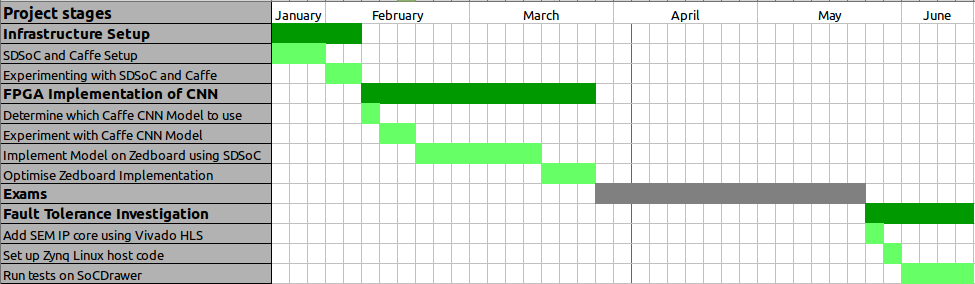
\includegraphics[width=1\textwidth]{../figures/gantt}

  \caption{A Gantt chart outlining an estimated timeline for the implementation plan \label{fig:gantt}}

\end{figure}

\subsection{Infrastrucure Setup}
\label{sec:ImpPlan-InfSetup}
\vspace{-12pt}

The work will be performed on a Ubuntu computer, and the first part of the project is setting up the necessary tools on the computer. The first tool to setup up is the Xilinx SDSoC development environment. SDSoC will be used to design the system. SDSoc is able to optimise and compile C, C++ or OpenCL source code for a Zynq system. The compiler generates software for the ARM core and, using an HLS tool, a bitstream for the FPGA. This allows the user to design the entire system, easily accelerating functions with the FPGA. SDSoc is a very powerful tool, facilitating the rapid development and design of firmware.

The other important tool to set up is called Caffe (or Convolutional Architecture for Fast Feature Embedding). This is a deep learning framework that can be used to design, train, optimise and test CNNs, with a focus on computer vision \cite{jia2014caffe}. Caffe also includes some examples of pre-trained CNN models that are ready for use. Using Caffe, it will be possible to generate C++ code for a CNN, which can then be implemented on the Zedboard system using SDSoc. This should be completed by the 31st of January, and some experiments will be performed using Caffe and SDSoC until the 3rd of February to build familiarity with the software.

\subsection{FPGA Implementation of a CNN}
\label{sec:ImpPlan-FPGAImplOfCnn}
\vspace{-12pt}

The next part of the project is implementing a CNN on the Zedboard platform. Using SDSoC, control software will be designed to run on the ARM processor, and the layers of the CNN will be implemented in HLS to run on the Programmable Logic. A pre-trained model of a CNN will be downloaded using Caffe and tested  on a computer, and then it will be implemented using SDSoC and tested on the Zedboard. Once this is complete, optimisation will be performed wherever possible, the literature concerning FPGA based CNN accelerators will be re-reviewed to check for ways to improve performance. It is expected that this should be complete by the 24th of March.

\subsection{Fault Tolerance Investigation}
\label{sec:ImpPlan-FaultTolInv}
\vspace{-12pt}

The final stage of the project is to perform experiments, in order to evaluate the system's suitability for space applications. Rather than creating SEUs with actual radiation, they can be simulated through fault injection \cite{FaultInjection}. An important tool in this process will be the Xilinx Soft Error Mitigation (SEM) Controller. The SEM IP core is able to perform SEU detection, correction, and classification, and can also simulate SEUs with error injection \cite{ManualSEM}. By adding the SEM core to the system using Xilinx's Vivado HLS tool, the system's resistance to SEUs can be tested and measured. 

The tests will be run using Zynq Linux host code. Xilinx provides a Linux image which can run on Zynq systems, including a kernel and a root file system. Using this, high quality results can be printed by the system as the tests are run. Once the setup is complete, the testing will begin. The FPGA has over 28K logic cells, so testing a reasonable number of SEU situations would take a very long time. In order to expedite the testing process, the experiments will be performed using an array of Zedboards, known the SoCDrawer. By running the tests in parallel, results can be gained much more quickly. This should be completed by the 14th of June.

\section{Evaluation Plan}
\label{sec:EvalPlan}
\vspace{-12pt}

Each of the two main deliverables of the project will be evaluated. This section will give details on how each deliverable will be tested, and how the success of each deliverable will be measured.

\subsection{FPGA Implementation of a CNN}
\label{sec:EvalPlan-FPGAImplOfCnn}
\vspace{-12pt}

The testing and critical assessment embedded CNN implementation is crucial to the success of the project. If this cannot be completed, or is completed  incorrectly, the rest of the project is jeapordised. If the CNN does not perform sufficiently well, the usefuleness of the project's results is diminished. Therefore, the FPGA CNN implementation will be throughly tested and examined.

There are two main criteria that the success of this deliverable will be evaluated on. These are the performance, measured in Giga Operations per second (GOp/s), and the resource efficiency, measured in Giga Operations per second per slice (GOp/s/Slice). Slices are a measure of FPGA resources, and are implemented differently on different FPGA families, but on a Zynq 7000, a slice is defined as four Look Up Tables (LUTs), and their associated flip-flops, mulitplexers and carry logic \cite{ManualZynq}. 

These criteria will be evaluated in comparison to results from literature. For example, Qui et al. implemented an FPGA accelerator with a overall performance of $136.97$ GOP/s and a $2.61\times 10^{-3}$ GOP/s/Slice. This is a very good result and achieving these values would be ideal. Another example, using a Zynq 7000 system and a CNN model called fpgaConvNet, is that described by Venieris et al., which achieved $12.73$ GOp/s and$4.5\times 10^{-4}$ GOp/s/Slice\cite{fpgaConvNet}. Given that this is on the same platform that I will use, this is a more realistic result to aim for. 

To confirm that the CNN has been successfully implemented, the classification accuracy will be tested. The accuracy of a CNN is typically meaured as top-1 accuracy and top-5 accuracy, which give the proportion of the testing data for which the correct class was assigned the highest probablilty and was in the highest 5 assigned probabilities respectively. This accuracy will depend on which CNN model is implemented, but as an example, the full precision Caffe AlexNet model acheives a top-1 accuracy of 56.82\% and a top-5 accuracy of 79.95\% \cite{fpgaCnnAccelerator}. The accuracies acheived by the FPGA implementation will depend greatly on which model we choose to implement, but if we chose AlexNet for example, we would expect to achieve accuracies close to these results.

Other criteria that may be evaluated are the total execution time, the total resource efficiency, the total power consumption and the power efficiency (GOp/W). There are articles which provide these values for their implementations\cite{ChenFpgaAccelerator}, against which I would compare my implementation's results.

\subsection{Fault Tolerance Investigation}
\label{sec:EvalPlan-FaultTolInv}
\vspace{-12pt}

The other deliverable to be assessed is the SEU tolerance. A good measure for this is Failure In Time (FIT), which is the number of failures that can be expected in $10^9$ hours of operation. This will be tested with the Xilinx SEM IP core and the SoCDrawer, as described in Section \ref{sec:ImpPlan-FaultTolInv}. This result will be analysed and used to evaluate the suitabillity of the system for space applications.

\section{Conclusion}
\label{sec:Conclusion}
\vspace{-12pt}

In this report, the outline of this project was presented. In Section \ref{sec:Background}, the target platform was defined, and important concepts concerning CNN structures, FPGA implementations, and FPGA applications in space were briefly described. Section \ref{sec:ProjSpec} gave the Project Specification, laying out the objectives of the project and what I expect to achieve. Section \ref{sec:ImpPlan} provided a plan of how each part of the project will be implemented, and what work needs to be done to achieve these objectives. Finally Section \ref{sec:EvalPlan} set out the metrics that will be used to determine whether each stage of the project has been successfully completed. 

\bibliography{interimReport_ref}
\bibliographystyle{ieeetr}
\nocite{*}


\end{document}